\documentclass[../../main/main.tex]{subfiles}
\graphicspath{{./figures/}}

\dominitoc
\faketableofcontents

\makeatletter
\renewcommand{\@chapapp}{\'Electrocin\'etique -- chapitre}
\makeatother

% \toggletrue{student}
% \HideSolutionstrue

\begin{document}
\setcounter{chapter}{3}

\chapter{Oscillateurs harmonique et amorti}

\vfill

\begin{prgm}
	\begin{tcb}*(ror)"know"{Savoirs}
		\begin{itemize}[label=$\diamond$, leftmargin=10pt]
			\item Analyser, sur des relevés expérimentaux, l’évolution de la forme des
			      régimes transitoires en fonction des paramètres caractéristiques.
			\item Prévoir l’évolution du système à partir de considérations
			      énergétiques.
			\item Écrire sous forme canonique l’équation différentielle afin
			      d’identifier la pulsation propre et le facteur de qualité.
			\item Décrire la nature de la réponse en fonction de la valeur du facteur
			      de qualité.
		\end{itemize}
	\end{tcb}

	\begin{tcb}*(ror)"how"{Savoir-faire}
		\begin{itemize}[label=$\diamond$, leftmargin=10pt]
			\item Établir et reconnaître l’équation différentielle qui caractérise un
			      oscillateur harmonique ; la résoudre compte tenu des conditions
			      initiales.
			\item Caractériser l’évolution en utilisant les notions d’amplitude, de
			      phase, de période, de fréquence, de pulsation.
			\item Réaliser un bilan énergétique.
			\item Déterminer la réponse détaillée dans le cas d’un régime libre ou
			      d’un système soumis à un échelon en recherchant les racines du
			      polynôme caractéristique.
			\item Déterminer un ordre de grandeur de la durée du régime transitoire
			      selon la valeur du facteur de qualité.
		\end{itemize}
	\end{tcb}
\end{prgm}

\vfill
\minitoc
\vfill

\newpage

Dans le chapitre précédent, nous avons vu des systèmes qui présentent un régime
transitoire caractérisé par des exponentielles croissantes ou décroissantes. En
combinant deux de ces composants, on trouve alors des régimes transitoires
caractérisé par une combinaison d'exponentielles, exprimée sous la forme de
fonctions sinusoïdales. Regardons un exemple.

\section{Oscillateurs harmoniques}
\subsection{Introduction harmonique}

\subsubsection{Signal sinusoïdal}

\begin{tcbraster}[raster columns=2, raster equal height=rows]
	\begin{tcb}[label=def:signsu](defi){Signal sinusoïdal}
		Un signal sinusoïdal est un signal de la forme
		\psw{
			\[
				\boxed{s(t) = A\cos(\wt + \f)}
			\]
		}
		$A$ est l'\textit{amplitude}, telle que
		\psw{
			\[
				A = \frac{s_{\max} - s_{\min}}{2}
			\]
		}
		$\wt +\f$ est la \textit{phase instantanée} du signal, avec
		\vspace*{-20pt}
		\begin{center}
			\begin{tikzpicture}[]
				\node[anchor=center] (name) at (0,0)
				{\textcolor{cornflowerblue}{$\w$}$t$+\textcolor{limegreen}{$\f$}};
				\node[inner sep=0] (datab) at ([shift={(0,3pt)}]name.south west) {};
				\node[inner sep=0] (biasb) at ([shift={(0,3pt)}]name.south east) {};
				\node[below left =.5cm and .5cm of datab, color=cornflowerblue] (data)
				{pulsation};
				\node[below right=.5cm and .5cm of biasb, color=limegreen] (bias)
				{phase initiale};
				\draw[-stealth] (data) -- (datab);
				\draw[-stealth] (bias) -- (biasb);
			\end{tikzpicture}
		\end{center}
		\tcbsubtitle{\fatbox{Unités}}
		La phase s'exprime en \textbf{radians}~; la pulsation en
		\textbf{$\si{rad.s^{-1}}$}.
	\end{tcb}
	\begin{tcb}[label=exem:graph](exem)'r'{Graphique}
		\begin{center}
			\switch{
				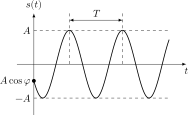
\includegraphics[width=\linewidth, draft=true]{ch8-fig1}
			}{
				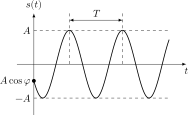
\includegraphics[width=\linewidth]{ch8-fig1}
			}
			\captionof{figure}{}
		\end{center}
		La pulsation représente la \textbf{vitesse avec de variation de la phase}.
		Pour une variation de $2\pi$ effectuée à la période $T$, on définit
		\psw{
			\[
				\boxed{\w = 2\pi/T = 2\pi f}
			\]
		}
		\vspace{-15pt}
	\end{tcb}
\end{tcbraster}

\subsubsection{Équation différentielle oscillateur harmonique}

\begin{tcbraster}[raster columns=2, raster equal height=rows]
	\begin{tcb}[label=prop:eqdiffoh](prop){Équation différentielle}
		Un oscillateur harmonique à un degré de liberté est un système dont
		l'évolution temporelle est décrite par une grandeur $x(t)$ solution
		d’une équation différentielle du type~:
		\psw{
		\[
			\boxed{ \dv[2]{x}{t} + \w_0{}^2x = \w_0{}^2x_{\rm eq}}
		\]
		}
		Avec $x_{\rm eq}$ la position d'équilibre du système et $\w_0$ la
		pulsation \textbf{propre}.
	\end{tcb}
	\begin{tcb}[label=prop:soluoh](prop)'r'{Solutions}
		La forme générale des solutions d'un oscillateur harmonique s'écrit de
		manière équivalente
		\psw{
			\begin{empheq}[box=\fbox]{gather*}
				x(t) = A'\cos(\w_0 t + \f) + x_{\rm eq}\\
				x(t) = A\cos(\w_0 t) + B\sin(\w_0 t) + x_{\rm eq}
			\end{empheq}
		}
		avec $A'$, $A$, $B$ des \textit{constantes d'intégration}.
	\end{tcb}
\end{tcbraster}

\subsubsection{Changement de variable~: de général à homogène}
\begin{tcb}[label=demo:chvar](rema)<lfnt>{Changement de variable}
	Au cours du chapitre précédent, nous avons vu la méthode pour résoudre
	des équations différentielles du premier ordre. Nous avons pu remarquer
	que les équations différentielles entre les échelons montants et
	descendants étaient en tout point similaire si ce n'est pour la présence
	ou non d'un second membre, impliquant la recherche d'une solution
	particulière ou non.

	Le changement de variable permet \textbf{d'éviter de
		chercher une solution particulière constante}.
\end{tcb}
\begin{tcb}[label=prop:chvar](prop){Changement de variable}
	Si $x(t)$ est solution de
	\psw{
	\[
		\boxed{ \dv[2]{x}{t} + \w_0{}^2x = \w_0{}^2x_{\rm eq}}
	\]
	}
	alors $y(t) = x(t) - x_{\rm eq}$ est solution de
	\psw{
		\[
			\boxed{ \dv[2]{y}{t} + \w_0{}^2y = 0}
		\]
	}
\end{tcb}
\begin{tcb}(appl)<lfnt>{}
	Résoudre l'équation du circuit RL montant par changement de variable.
	\tcblower
	\psw{
		L'équation différentielle totale s'écrit
		\[
			\boxed{
				\dv{i}{t} + \frac{1}{\tau}i =
				\frac{1}{\tau}\frac{E}{R}
			}
			\Lra
			\dv{i}{t} + \frac{i-\frac{E}{R}}{\tau} = 0
		\]
		On peut donc définir
		\[
			i_h(t) = i(t) - \frac{E}{R} \quad \Ra \quad \dv{i_h}{t} = \dv{i}{t} + 0
		\]
		donc $i_h$ est solution de
		\[
			\dv{i_h}{t} + \frac{i_h}{\tau} = 0
		\]
		de solution générale
		\[
			i_h(t) = A\exr^{-t/\tau}
		\]
		On peut directement chercher l'expression de $A$ par CI~:
		\[
			i_h(0) = \underbracket[1pt]{i(0)}_{=0} - \frac{E}{R} = A
		\]
		Et en ré-isolant $i(t)$, on trouve bien
		\[
			\boxed{i(t) = \frac{E}{R}\left( 1 - \exr^{-t/\tau} \right)}
		\]
	}
	\vspace{-15pt}
\end{tcb}

\subsubsection{Exemple expérimental~: l'oscillateur LC}

Soit le circuit suivant sous un échelon de tension descendant. On observe la
tension $u_C(t)$ avec un oscilloscope dont la courbe est représentée à droite.
\textbf{Une simulation est disponible en
	ligne\ftn{\url{https://tinyurl.com/yl9rvpqg}}}.

\begin{minipage}{0.50\linewidth}
	\begin{center}
		\switch{
			\includegraphics[width=\linewidth, draft=true]{lc_descendant}
		}{
			\includegraphics[width=\linewidth]{lc_descendant}
		}
		\captionof{figure}{}
	\end{center}
\end{minipage}
\begin{minipage}{0.50\linewidth}
	\begin{center}
		\switch{
			\includegraphics[width=.7\linewidth,
				draft=true]{carac-lc_descendant-harmonique-intro}
		}{
			\includegraphics[width=.7\linewidth]{carac-lc_descendant-harmonique-intro}
		}
		\captionof{figure}{}
	\end{center}
\end{minipage}
On remarque que la tension aux bornes du condensateur réalise des
d'oscillations sinusoïdales amorties. En fonction des valeurs des
caractéristiques des composants, on trouve~:
\begin{itemize}
	\item Pour $C_1 = \SI{80}{nF}$ et $L_1 = \SI{43}{mH}$, un période de $T_1 =
		      \SI{364}{\micro s}$~;
	\item Pour $C_2 = \SI{20}{nF}$ et $L_2 = \SI{43}{mH}$, un période de $T_2 =
		      \SI{184}{\micro s}$~;
\end{itemize}

\begin{tcb}(expe){Analyse}
	Lorsque l'on excite le système LC, la tension aux bornes du condensateur
	oscille de façon régulière et sinusoïdale, avec une période qui ne dépend pas
	de l'amplitude de l'excitation mais des caractéristiques de l'oscillateur
	(capacité du condensateur et inductance de la bobine).
\end{tcb}

C'est ce que nous allons maintenant démontrer analytiquement.

\subsection{Oscillateur harmonique électrique~: circuit LC régime
	libre}\label{sec:lclibre}

\subsubsection{Présentation}

\begin{minipage}[c]{.6\linewidth}
	\begin{itemize}
		\item Il est constitué de l'association en série d'une bobine et d'un
		      condensateur idéaux.
		\item \textbf{On suppose le condensateur initialement chargé}~:
		      \fbox{$u_C(0^-) = E$ \underline{et} $i(0^-) = 0$} (condensateur chargé
		      $\equiv$ interrupteur ouvert).
		\item À $t=0$, on coupe le générateur.
	\end{itemize}
\end{minipage}
\hfill
\begin{minipage}[c]{.35\linewidth}
	~
	\begin{center}
		\switch{
			\includegraphics[width=.9\linewidth, draft=true]{lc_descendant-intens}
		}{
			\includegraphics[width=.9\linewidth]{lc_descendant-intens}
		}
		\captionof{figure}{}
	\end{center}
\end{minipage}

\subsubsection{Équation différentielle du circuit}
\begin{tcb}[label=demo:eqdiffrc](demo)<lfnt>{Équation diff. LC}
	Avec la loi des mailles,
	\psw{
		\begin{DispWithArrows*}[]
			u_L + u_C &= 0
			\Arrow{$\DS u_L = L \dv{i}{t}$\\ et $\DS i = C \dv{u_C}{t}$}
			\\\Lra
			LC \dv[2]{u_C}{t} + u_C          &= 0
			\Arrow{forme canonique}
			\\
			\Lra \dv[2]{u_C}{t} + \frac{1}{LC}u_C &= 0
		\end{DispWithArrows*}
		D'où le résultat. $L$ assure $i(0^+) = 0$ et $C$ assure $u_C(0^+) = E$
		par continuité.
	}
\end{tcb}
\begin{tcb}[label=prop:eqdiffrc, sidebyside, righthand ratio=.4](prop){Équation diff. LC}
	L'équation différentielle de la tension $u_C(t)$ aux bornes d'un
	condensateur dans un circuit LC en décharge est
	\psw{
		\[
			\boxed{\dv[2]{u_C}{t} + \w_0{}^2u_C = 0}
		\]
	}
	avec \fbox{$\w_0 = \frac{1}{\sqrt{LC}}$} la pulsation propre.
	\tcblower
	Les conditions initiales (continuité de $u_C$ aux bornes de $C$
	et de $i$ traversant $L$) sont
	\psw{
		\begin{empheq}[box=\fbox]{gather*}
			u_C(0^-) = u_C(0^+) = E\\
			i(0^-) = i(0^+) = 0
		\end{empheq}
	}
\end{tcb}

\begin{tcb}[label=rema:unité](appl){Unité de $\w_0$}
	On peut vérifier à cette étape que $\w_0$ est bien homogène à l'inverse d'un
	temps. Pour ça, deux manières~:

	\begin{isd}[sidebyside align=top]
		\tcbsubtitle{\fatbox{Analyse directe}}
		Sachant que $RC$ et $L/R$ sont des temps (cf.\ chapitre précédent)~:
		\psw{
			\begin{align*}
				w_0{}^2 = \frac{1}{LC} =
				\frac{\textcolor{cornflowerblue}{R}}
				{\textcolor{cornflowerblue}{L}\textcolor{orange}{RC}}
				= \underbrace{\left[ \frac{L}{R}
						\right]^{-1}}_{\si{s^{-1}}}\times
				\underbrace{\left[ RC \right]^{-1}}_{\si{s^{-1}}}
			\end{align*}
			Et on a bien $\w_0{}^2$ en \si{s^{-2}}, et donc $\w_0$ en \si{s^{-1}},
			les radians n'ayant pas de dimension.
		}
		\tcblower
		\tcbsubtitle{\fatbox{Analyse indirecte}}
		En effet, l'équation différentielle est forcément une équation homogène.
		Ainsi
		\psw{
			\begin{equation*}
				\left[ \dv[2]{u_C}{t} \right] =
				\frac{\left[u_C\right]}{\left[\dt\right]^2}\\
				= \frac{\si{V}}{\si{s^2}}
			\end{equation*}
			et l'autre terme doit avoir la même unité~:
			\begin{equation*}
				\left[ w_0{}^2u_C \right] = \left[ w_0 \right]^2\times \left[
					u_C \right]\\
				= \si{V.s^{-2}}
			\end{equation*}
			On en déduit que $\w_0{}^2$ est de dimension \si{s^{-2}}, d'où la
			dimension de $\w_0$.
		}
	\end{isd}
\end{tcb}

\subsubsection{Résolution de l'équation différentielle et graphique}
\begin{tcb}[label=demo:rcsolu](demo){Solutions LC série descendant}
	L'équation étant déjà homogène, on écrit la forme générale~:
	\psw{
		\[
			u_C(t) = A\cos(\w_0 t) + B\sin(\w_0 t)
		\]
	}
	\vspace{-15pt}
	\begin{itemize}
		\item On trouve $A$ avec la première condition initiale~:
		      \psw{
			      \[
				      u_C(0) = A\cos(0) + B\sin(0) = A
				      \qet
				      u_C(0) = E
				      \quad \Ra \boxed{A = E}
			      \]
		      }
		      \vspace{-15pt}
		\item On trouve $B$ avec la seconde condition initiale~:
		      \psw{
			      \begin{gather*}
				      \dv{u_C}{t} = -A\w_0\sin(\w_0t) + B\w_0\cos(\w_0t)
				      \Ra \dv{u_C}{t}\/(0) = B\w_0
				      \\
				      \text{et} \quad
				      i(0) = 0 = C \dv{u_C}{t}\/(0) = CB\w_0
				      \quad \Ra \boxed{B = 0}
			      \end{gather*}
		      }
		      \vspace{-15pt}
	\end{itemize}
	On obtient ensuite $i$ avec la relation courant-tension~:
	\psw{
		\[
			i(t) = C \dv{u_c}{t} = -CE \w_0 \sin(\w_0t)
		\]
	}
	\vspace{-15pt}
\end{tcb}
\begin{tcbraster}[raster columns=2, raster equal height=rows]
	\begin{tcb}[label=prop:ucsolu](prop){Solution de l'équation
				différentielle LC}
		La solution de l'équation différentielle de la tension $u_C(t)$
		d'un circuit LC en décharge avec $u_C(0) = E$ et l'intensité en
		découlant sont
		\psw{
			\begin{empheq}[box=\fbox]{gather*}
				u_C(t) = E\cos(\w_0t)\\
				i(t) = -CE\w_0\sin(\w_0t)
			\end{empheq}
		}
	\end{tcb}
	\begin{tcb}[width=\linewidth](exem)'r'{Graphique}
		\begin{center}
			\switch{
				\includegraphics[width=\linewidth,
					draft=true]{carac-lc_descendant-harmonique}
			}{
				\includegraphics[width=\linewidth]{carac-lc_descendant-harmonique}
			}
			\captionof{figure}{}
		\end{center}
	\end{tcb}
\end{tcbraster}

\subsubsection{Bilan énergétique}
\begin{tcb}[label=demo:rcenerg-charge](demo){Bilan d'énergie}
	On fait un bilan de puissances avec la loi des mailles multipliée par $i$~:
	\psw{
		\begin{DispWithArrows*}
			u_Ci + u_Li = 0
			\Arrow{$i = C \dv{u_C}{t}$\\et $u_L = L \dv{i}{t}$}
			\\
			\Lra u_C\times C \dv{u_C}{t} + L \dv{i}{t}\times i = 0
			\Arrow{$f \times f' = \left( \frac{1}{2}f^{2} \right)'$}
			\\
			\Lra \dv{}{t} \left( \frac{1}{2}Cu_C{}^2 + \frac{1}{2}Li^2 \right) = 0
		\end{DispWithArrows*}
		On identifie l'intérieur de la parenthèse à l'énergie du système (car
		par définition $\Pc = \dv{\Ec}{t}$) pour avoir la propriété.
	}
\end{tcb}
\begin{tcbraster}[raster columns=2, raster equal height=rows]
	\begin{tcb}[label=prop:lcenerg-décharge](prop){Bilan d'énergie}
		L'énergie emmagasinée dans le circuit est
		\psw{
		\[
			\boxed{\Ec = \frac{1}{2}Cu_C{}^2 + \frac{1}{2}Li^2}
		\]
		}
		Elle est \textbf{conservée à chaque instant} et résulte de l'\textbf{échange
			périodique} d'énergie entre le condensateur et la bobine.
	\end{tcb}
	\begin{tcb}[width=\linewidth](exem)'r'{Graphique}
		\begin{center}
			\switch{
				\includegraphics[width=\linewidth, draft=true]{carac-lc_descendant-bilan}
			}{
				\includegraphics[width=\linewidth]{carac-lc_descendant-bilan}
			}
			\captionof{figure}{}
		\end{center}
	\end{tcb}
\end{tcbraster}

\begin{tcb}[label=impl](impl){Vérification conservation de l'énergie}
	On vérifie avec les expressions analytiques trouvées, sachant que
	$\w_0{}^2 = (LC)^{-1}$~:
	\psw{
		\begin{align*}
			\frac{1}{2}Cu_C{}^2 & = \frac{1}{2}CE^2\cos^2(\w_0t)
			\\
			\text{et} \quad
			\frac{1}{2}Li^2     & =
			\frac{1}{2}\underbracket[1pt]{LC^{2}\w_0{}^2}_{=C}E^2\sin^2(\w_0t)
			\\\Ra
			\Ec                 & = \frac{1}{2}CE^2 \left( \cos^2(\w_0t) + \sin^2(\w_0t) \right)
		\end{align*}
		Soit
		\begin{equation*}
			\boxed{\Ec = \frac{1}{2}CE^2 = \text{cste}}
		\end{equation*}
	}
\end{tcb}
\begin{tcb}[label=impo:amortissement](impo){Résultat}
	On retrouve bien des oscillations de la tension aux bornes de $u_C$ comme dans
	l'approche expérimentale, avec une période $T_0 = \frac{2\pi}{\w_0} =
		2\pi\sqrt{LC}$ qui augmente avec $L$ et $C$.
	\bigbreak
	Il n'y a donc \textbf{pas d'amortissement ici}~! En effet les composants
	utilisés ici sont idéaux, et conservent totalement l'énergie, il n'y a pas de
	raison d'en perdre.
	\bigbreak
	Il y a eu une simplification que l'on effectue souvent en mécanique~:
	\textbf{on a négligé les effets dissipatifs}. Regardons comment ça se traduit
	pour un exemple mécanique.
\end{tcb}

\subsection{Exemple harmonique mécanique~: ressort horizontal libre}

\subsubsection{Introduction}

\begin{tcb}[label=defi:ressortdef, sidebyside, righthand ratio=.5](defi){Force de
			rappel d'un ressort}
	Soit le système masse-ressort horizontal représenté ci-contre. Le ressort se
	déforme sous l'effet d'une contrainte en stockant l'énergie donnée, qu'il
	libère en reprenant sa forme quand la contrainte s'arrête. On définit la
	force de rappel du ressort par~:
	\psw{
		\begin{equation*}
			\boxed{\vv*{F}{\rm rappel} = -k(\ell - \ell_0)\ux}
		\end{equation*}
	}
	\vspace{-15pt}
	\begin{itemize}
		\item $k > 0$ la \textbf{constante de raideur}~;
		\item $\ell_0$ sa \textbf{longueur à vide}~;
		\item $\ux$ un vecteur unitaire \ftn{$ \left\Vert \ux \right\Vert = 1$}
		      dirigé selon $x$.
	\end{itemize}
	\tcbsubtitle{\fatbox{Unité}}
	\psw{
	$k$ en $\si{N.m^{-1}}$ ($[\vv{F}] = [k][\ell]$)
	}
	\tcblower
	\begin{center}
		\includegraphics[width=\linewidth]{ressort_def}
		\captionof{figure}{}
	\end{center}
	Si $\ell > \ell_0$, on a bien une force dirigée selon $-\ux$, (situation
	\circled{2}), sinon dirigée selon $+\ux$.
\end{tcb}

\subsubsection{Présentation}
\begin{tcb}[label=def:ressortlibre, sidebyside, righthand ratio=.5](defi){Situation
			initiale et bilan des forces}
	\begin{itemize}[label=$\diamond$, leftmargin=10pt]
		\bitem{Système~:} \{point M\} de masse $m$, accroché à un \textbf{ressort
			idéal sans frottements}
		\bitem{Référentiel~:} $\Rc\ind{sol}(O',x,y,t)$ supposé galiléen
		\bitem{Repère~:} $(\Or', \ux, \uy)$ (voir schéma)
		\bitem{Repérage~:}
		\vspace{-15pt}
		\begin{center}
			\fbox{Soit $x (t) = \ell(t) - \ell_0$ la position de la masse}
		\end{center}
		\[
			{\rm O'M} = x(t)\ux~; \vf = \xp(t)\ux~; \af = \xpp(t)\ux.
		\]
		\bitem{Origine initiale~:} ${\rm O'M}(0) = x_0 >0$
		\bitem{Vitesse initiale~:} $\vf(0) = \of$
	\end{itemize}
	\tcblower
	\begin{center}
		\switch{
			\includegraphics[width=\linewidth, draft=true]{ressort_libre}
		}{
			\includegraphics[width=\linewidth]{ressort_libre}
		}
		\captionof{figure}{}
	\end{center}
	\begin{itemize}[label=$\diamond$, leftmargin=10pt]
		\bitem{Bilan des forces~:}
		\psw{
			\[
				\begin{array}{ll}
					\textbf{Poids}            & \Pf = m\gf = -mg \uy \\
					\textbf{Réaction normale} & \Rf = R\uy           \\
					\textbf{Force de rappel}  & \Ff = -kx (t)\ux
				\end{array}
			\]
		}
	\end{itemize}
\end{tcb}

\subsubsection{Équation différentielle et solution}

\begin{tcb}[label=demo:solreslibre, sidebyside](demo){Équation différentielle et solution}
	\tcbsubtitle{\fatbox{Équation}}
	La deuxième loi de \textsc{Newton}, ou \textbf{principe fondamental de la
		dynamique} (PFD) donne~:
	\psw{
		\begin{gather*}
			\dv{\pf}{t} = m\af = \Pf + \vv{R} + \Ff\\
			\Lra m
			\mqty(
			\dv[2]{x}{t} \\
			0
			)
			=
			\mqty(
			-kx \\
			-mg + R
			)
		\end{gather*}
	}
	Sur l'axe $\ux$\ftn{La projection sur $\uy$ montre que la réaction du support
		compense le poids.} on trouve alors
	\psw{
		\[
			m \dv[2]{x}{t} + kx = 0 \Lra \boxed{\dv[2]{x}{t} + \w_0{}^{2}x = 0}
		\]
	}
	\tcblower
	\tcbsubtitle{\fatbox{Solution}}
	On écrit la forme générale~:
	\psw{
		\[
			x(t) = A\cos(\w_0 t) + B\sin(\w_0 t)
		\]
	}
	\vspace{-15pt}
	\begin{itemize}
		\item On trouve $A$~:
		      \psw{
			      \[
				      x(0) = A\cos(0) + B\sin(0) = A
				      \qet
				      x(0) = x_0
				      \quad \Ra \boxed{A = x_0}
			      \]
		      }
		      \vspace{-15pt}
		\item On trouve $B$~:
		      \psw{
			      \begin{gather*}
				      \dv{x}{t} = -A\w_0\sin(\w_0t) + B\w_0\cos(\w_0t)
				      \Ra
				      \dv{x}{t}\/(0) = B\w_0
				      \\
				      \text{et} \quad
				      v(0) = 0 = \dv{x}{t}\/(0) = B\w_0
				      \quad \Ra \boxed{B = 0}
			      \end{gather*}
		      }
		      \vspace{-15pt}
	\end{itemize}
	On obtient ensuite $v$ avec la relation vitesse-position.
\end{tcb}
\begin{tcb}[label=prop:eqdiffreslibre, sidebyside](prop){Équation et solution}
	La position $x$ de la masse et la longueur $\ell$ du ressort sont régies
	par~:

	\begin{empheq}[box=\fbox]{gather*}
		\dv[2]{x}{t} + \w_0{}^2x = 0
		\Lra \dv[2]{\ell}{t} + \w_0{}^2\ell = \w_0{}^2\ell_0
	\end{empheq}

	Avec $\w_0 = \DS \sqrt{\frac{k}{m}}$. $\ell_0$ est donc la longueur
	d'équilibre du système.
	\tcblower
	La position $x$ et la vitesse $v$ ont pour expression
	\begin{empheq}[box=\fbox]{gather*}
		x(t) = x_0\cos(\w_0t)\\
		v(t) = -x_0\w_0\sin(\w_0t)
	\end{empheq}
\end{tcb}
\begin{tcb}[label=rema:ressortlibre, sidebyside](rema){Analogie LC-ressort}
	Alors qu'on partait d'un système \textit{a priori} totalement différent, on
	remarque que la physique des deux systèmes sont rigoureusement équivalentes
	puisque \textbf{régies par la même équation différentielle}. On observe une
	oscillation du ressort autour d'une position d'équilibre, ici $x=0
		\Lra \ell = \ell_0$.
	\tcblower
	On peut donc associer $u_C$ à $x$ et $i$ à $v$, étant donné que pour un
	condensateur $i = C \dv{u_C}{t}$ et que $v = \dv{x}{t}$. Ainsi, \textbf{les
		échanges énergétiques sont les mêmes} entre l'énergie emmagasinée dans la
	déformation du ressort et l'énergie cinétique de la masse comme on va le
	voir juste après.
\end{tcb}

\subsubsection{Bilan énergétique}

\begin{tcbraster}[raster columns=2, raster equal height=rows]
	\begin{tcb}[label=def:emeca](defi){Énergies potentielle élastique et mécanique}
		Le ressort emmagasine une énergie \textit{potentielle} lors de sa
		déformation, telle que
		\[\boxed{\Ec_{p\rm, el} = \frac{1}{2}k(\ell-\ell_0)^2 = \frac{1}{2}kx^2}\]
		On définit alors l'énergie mécanique totale $\Ec_m$ du système par
		\[\boxed{\Ec_m = \Ec_c + \Ec_p}\]
		avec, évidemment, $\Ec_c = \frac{1}{2}mv^2$.
	\end{tcb}
	\begin{tcolorbox}[blankest, raster multicolumn=1, space to=\myspace]
		\begin{tcbraster}[raster columns=1]
			\begin{tcb}[label=prop:emecacons](prop){Conservation énergie}
				Dans le système masse-ressort horizontal sans frottements, l'énergie
				mécanique est conservée.
			\end{tcb}
			\begin{tcb}[label=demo:emecacons](demo){Conservation énergie}
				À partir de l'équation différentielle on multiplie par $\dv{x}{t}$ et on
				utilise que $ff' = (\frac{1}{2}f^2)'$ pour $f$ une fonction~:
				\begin{gather*}
					m \dv[2]{x}{t} \dv{x}{t} + kx \dv{x}{t} = 0\\
					\Lra \dv{}{t} \left( \frac{1}{2}m \left( \dv{x}{t} \right)^2 +
					\frac{1}{2}kx^2 \right) = 0
				\end{gather*}
				On a bien $ \frac{1}{2}mv^2 + \frac{1}{2}kx^2 = \Ec_m$ conservé.
			\end{tcb}
		\end{tcbraster}
	\end{tcolorbox}
	\begin{tcb}[label=impl](impl){Vérification}
		On vérifie avec les expressions analytiques trouvées, sachant que
		$\w_0{}^2 = \frac{k}{m}$~:
		\begin{gather*}
			\frac{1}{2}kx^2 = \frac{1}{2}kx_0{}^2\cos^2(\w_0t)\\
			\frac{1}{2}mv^2 =
			\frac{1}{2}\underbrace{m\w_0{}^2}_{=k}x_0{}^2\sin^2(\w_0t)\\
			\Ra \Ec_m = \frac{1}{2}kx_0{}^2 \left( \cos^2(\w_0t) +
			\sin^2(\w_0t) \right)
		\end{gather*}
		Soit
		\begin{equation*}
			\boxed{\Ec_m = \frac{1}{2}kx_0{}^2 = \text{cste}}
		\end{equation*}
	\end{tcb}
	\begin{tcb}[width=\linewidth](exem){Graphique}
		\begin{center}
			\includegraphics[width=\linewidth]{carac-ressort_libre-bilan}
		\end{center}
	\end{tcb}
\end{tcbraster}

\vspace*{-20pt}
\subsubsection{Analyse correspondance}
\begin{tcb}[width=\linewidth, sidebyside, righthand ratio=.4, hand](exem){Visualisation}

	Il est utile d'observer la physique des systèmes oscillants non pas dans
	un espace (grandeur, temps) mais dans un espace \textbf{(grandeur,
		dérivée)}, qui permet plus rapidement de sonder son évolution. Par
	exemple, le ressort lâché à $x_0$ et $v_0=0$ voit sa position diminuer
	et sa vitesse augmenter (algébriquement) jusqu'à ce qu'il passe par sa
	position d'équilibre ($x=0$) avec une vitesse extrémale $v_{\min}$,
	avant de se comprimer en perdant de sa vitesse. Comme il n'y a
	\textbf{pas de perte dans cette étape}, elle se répète
	\textbf{symétriquement} en revenant à son point de départ.

	\tcblower
	\begin{center}
		\includegraphics[width=\linewidth]{carac-ressort_libre-xy}
	\end{center}
\end{tcb}

\begin{tcb}[label=impo:harmotoamorti](impo){Conclusion}

	En réalité, les \textbf{frottements en mécanique existent}, et à chaque
	étape le système masse-ressort perd de l'énergie dans la dissipation par
	frottement créant de la chaleur. On va donc avoir une \textbf{trajectoire
		amortie} plus ou moins fortement. Dans le cas électrique, c'est la
	\textbf{résistance que nous avions négligée} alors qu'elle existe toujours~:
	notamment la bobine réelle est composée d'une bobine idéale et d'une
	résistance en série. C'est la résistance qui va \textbf{dissiper l'énergie}
	de l'oscillateur harmonique LC sous forme de chaleur par effet
	\textsc{Joule} et amortir l'oscillation de $u_C$. Nous allons donc étudier
	le circuit $RLC$ dans la suite.
\end{tcb}

\subsection{Complément~: circuit LC montant}

\subsubsection{Présentation}
\begin{tcb}[label=def:echelonC, sidebyside, righthand width=.4\linewidth](defi)
	{situation initiale}

	Le montage est représenté ci-contre. Il est constitué de l'association en
	série d'une bobine et d'un condensateur idéaux alimentés par un générateur
	de tension fixe $E$. \textbf{On suppose le condensateur initialement
		déchargé}~: \fbox{$u_C(0^-) = 0$}, et on ferme l'interrupteur à $t=0$, soit
	\fbox{$i(0^-) = 0$}.

	\tcblower
	\begin{center}
		\includegraphics[width=.65\linewidth]{lc_montant}
	\end{center}
\end{tcb}

\vspace*{-15pt}
\subsubsection{Équation différentielle du circuit}
\begin{tcbraster}[raster columns=2, raster equal height=rows]
	\begin{tcb}[label=prop:eqdiffrc](prop){Équation diff. LC}
		L'équation différentielle de la tension $u_C(t)$ aux bornes d'un
		condensateur dans un circuit LC en charge est
		\[ \boxed{\dv[2]{u_C}{t} + \w_0{}^2u_C = \w_0{}^2E}\]
		avec \fbox{$\w_0 = \frac{1}{\sqrt{LC}}$} la pulsation propre.
		\tcblower
		Les conditions initiales (continuité de $u_C$ aux bornes de $C$
		et de $i$ traversant $L$) sont
		\begin{empheq}[box=\fbox]{gather*}
			u_C(0^-) = u_C(0^+) = 0\\
			i(0^-) = i(0^+) = 0
		\end{empheq}
	\end{tcb}
	\begin{tcb}[label=demo:eqdiffrc](demo){Équation diff. LC}
		Avec la loi des mailles,
		$$u_L + u_C = E$$
		Ensuite, \textbf{en convention récepteur} on a~:
		$\DS u_L = L \dv{i}{t}$ et $\DS i = C \dv{u_C}{t}$
		\begin{gather*}
			L \dv{i}{t} + u_C                                = E
			\Lra LC \dv[2]{u_C}{t} + u_C          = E\\
			\Lra \dv[2]{u_C}{t} + \frac{1}{LC}u_C = \frac{1}{LC}E
		\end{gather*}

		D'où le résultat. $L$ assure $i(0^+) = 0$ et $C$ assure $u_C(0^+) = E$
		par continuité.
	\end{tcb}
\end{tcbraster}

\subsubsection{Résolution de l'équation différentielle et graphique}
\begin{tcbraster}[raster columns=2, raster equal height=rows]
	\begin{tcolorbox}[blankest, raster multicolumn=1, space to=\myspace]
		\begin{tcbraster}[raster columns=1]
			\begin{tcb}[label=prop:ucsolu](prop){Solution de l'équation
						différentielle LC}
				La solution de l'équation différentielle de la tension $u_C(t)$
				d'un circuit LC en charge avec $u_C(0) = 0$ et l'intensité en
				découlant sont
				\begin{empheq}[box=\fbox]{gather*}
					u_C(t) = E(1 - \cos(\w_0t))\\
					i(t) = CE\w_0\sin(\w_0t)
				\end{empheq}
			\end{tcb}
			\begin{tcb}[width=\linewidth](exem){Graphique}
				\begin{center}
					\includegraphics[width=\linewidth]{carac-lc_montant-harmonique}
				\end{center}
			\end{tcb}
		\end{tcbraster}
	\end{tcolorbox}
	\begin{tcb}[label=demo:rcsolu](demo){Solution LC série}
		D'après la propriété \ref{prop:chvar}, on sait que $u_C - E$ est
		solution de l'équation homogène associée, donc on a
		\[u_C(t) - E = A\cos(\w_0 t) + B\sin(\w_0 t)\]

		On trouve alors $A$ avec la première condition initiale~:
		$u_C(0^+) = 0$. En effet,
		\[u_C(0) - E = A\cos(0) + B\sin(0) = A\]
		donc $A=-E$.\smallbreak

		On trouve $B$ avec la seconde condition initiale~: $i(0^+) = 0 = C
			\dv{u_C}{t}$. En effet,
		\begin{gather*}
			\dv{u_C}{t} = -A\w_0\sin(\w_0t) + B\w_0\cos(\w_0t)\\
			\Ra \dv{u_C}{t} (0) = B\w_0
		\end{gather*}
		Donc $B = 0$ ($\w_0 \neq 0$), et $u_C - E = -E\cos(\w_0t)$. On obtient
		ensuite $i$ avec la relation courant-tension.
	\end{tcb}
	\begin{tcb}[label=rema:lccharge](rema){Valeur de $u_C$}
		On remarque aisément que $u_C$ atteint $2E$ par moment, ce qui pourrait
		paraître dérangeant puisqu'on donne une tension $E$ au système. En
		réalité ceci est tout à fait normal puisque $u_L = L\dv{i}{t}$ prend des
		valeurs négatives quand $i$ diminue~: la somme des deux fait bien $E$.
		On peut réaliser un bilan d'énergie pour vérifier que $\Ec_g =
			CE^2(1-\cos(\w_0t)) = \Ec_C + \Ec_L$, voir graphique ci-contre.
	\end{tcb}
	\begin{tcb}[width=\linewidth](exem){Bilan d'énergie}
		\begin{center}
			\includegraphics[width=\linewidth]{carac-lc_montant-bilan}
		\end{center}
	\end{tcb}
\end{tcbraster}

\subsubsection{Intérêt oscillateur harmonique}

Le principal intérêt de l'observation régulière d'une oscillation est la mesure
du temps. Une excitation quelconque (comme un échelon) produit un phénomène se
reproduisant à intervalle régulier et fait alors apparaître un étalon
temporel. Ce principe est utilisé~:
\begin{itemize}
	\item dans les horloges mécaniques à balancier~: on exploite le mouvement
	      régulier du pendule~;
	\item dans les horloges à ressort~: la période est liée au rapport de
	      l'inertie et de la raideur du système~;
	\item dans les horloges électroniques~: un cristal de quartz dont la
	      fréquence d'oscillation est précisément connue (en général une puissance
	      de 2 en Hz)~;
	\item dans les horloges atomiques~: on utilise la régularité des
	      oscillations des ondes électromagnétiques absorbées par un atome.
	      L'actuelle définition de la seconde est basée sur le fonctionnement
	      d'une horloge atomique.
\end{itemize}

\section{Oscillateurs amortis}
\subsection{Introduction amorti}

\subsubsection{Évolutions en régime libre, exemple RLC}

\begin{minipage}{0.60\linewidth}
	En reprenant les résultats de la subsection~\ref{sec:lclibre}, nous devrions en
	réalité observer que les oscillations dans le circuit s’atténuent. Plus
	quantitativement, avec le circuit suivant on a~:
\end{minipage}
\begin{minipage}{0.40\linewidth}
	\begin{center}
		\includegraphics[width=.7\linewidth]{rlc_descendant}
	\end{center}
\end{minipage}

\begin{itemize}
	\item Lorsque la résistance est petite~: on observe plusieurs oscillations.
	      Nous avons câblé un circuit avec $L = \SI{43}{mH}$ et $C = \SI{20}{nF}$.
	      On observe une série d’oscillations à la période $T \approx \SI{184}{\micro
			      s}$. On observe environ 25 oscillations lorsque $R \approx
		      \SI{60}{\ohm}$ (résistance interne du GBF + de la bobine), 9
	      oscillations lorsque $R \approx \SI{180}{\ohm}$, 5 oscillations lorsque
	      $R \approx \SI{500}{\ohm}$.
\end{itemize}
\begin{minipage}{0.45\linewidth}
	\begin{center}
		\includegraphics[width=\linewidth]{carac-rlc-15}
	\end{center}
\end{minipage}
\hfill
\begin{minipage}{0.45\linewidth}
	\begin{center}
		\includegraphics[width=\linewidth]{carac-rlc-3}
	\end{center}
\end{minipage}

\begin{itemize}
	\item Lorsque la résistance est plus grande~: les oscillations
	      disparaissent. Lorsque $R \approx \SI{2,9}{k\ohm}$, on observe un régime
	      transitoire dont la durée est d’environ $\SI{250}{\micro s}$ (à 95\%).
	      Lorsque $R \approx \SI{7.5}{k\ohm}$, on observe un régime transitoire
	      plus long, d’environ \SI{420}{\micro s}.
\end{itemize}
\begin{minipage}{0.45\linewidth}
	\begin{center}
		\includegraphics[width=\linewidth]{carac-rlc-05}
	\end{center}
\end{minipage}
\hfill
\begin{minipage}{0.45\linewidth}
	\begin{center}
		\includegraphics[width=\linewidth]{carac-rlc-02}
	\end{center}
\end{minipage}

\begin{tcb}(expe){Analyse}
	Lorsque l'on excite le système RLC, la tension aux bornes du condensateur
	varie selon la valeur de la résistance avec plus ou moins d'oscillations,
	jusqu'à n'avoir aucune oscillation quand $R \gg 1$. La période ne cesse
	d'augmenter quand $R$ augmente.
\end{tcb}

\subsubsection{Équation différentielle}

\begin{tcbraster}[raster columns=2, raster equal height=rows]
	\begin{tcb}[label=prop:eqdiffoh](prop){Équation différentielle}
		Un oscillateur amorti à un degré de liberté est un système dont l'évolution
		temporelle est décrite par une grandeur $x(t)$ solution d'un équation
		différentielle du type~:
		\[ \boxed{ \dv[2]{x}{t} + \frac{\w_0}{Q} \dv{x}{t} + \w_0{}^2x = \w_0{}^2x_{\rm eq}}\]
		Avec $x_{\rm eq}$ la position d'équilibre, $\w_0$ la pulsation
		\textbf{propre}, et $Q >0$ le \textbf{facteur de qualité}, sans dimension.
	\end{tcb}
	\begin{tcb}[label=impl:eqdiffamorti](impl){Analyse de l'équation}
		Par lecture de cette équation, avec $Q$ sans dimension on retrouve que
		$\w_0$ s'exprime en \si{s^{-1}} car $\dv{x}{t}$ est de dimension
		\si{[x].s^{-1}}.\bigbreak
		De plus, on remarque que \textbf{plus $Q$ est élevé}, plus le terme
		d'ordre 1 est négligeable devant les autres, donc \textbf{plus on se
			rapproche de l'harmonique}. Le facteur de qualité traduit donc à quel
		point le système est presque idéal.
	\end{tcb}
\end{tcbraster}

\subsubsection{Équation caractéristique et régimes de solutions}
\begin{tcbraster}[raster columns=2, raster equal height=rows]
	\begin{tcb}[label=def:eqcarac](defi){Équation caractéristique}
		Pour résoudre une équation différentielle, on suppose une solution de la
		forme $x(t) = K\exp(rt)$ avec $r \in \Cb$. En injectant cette
		expression dans l'équation différentielle, on obtient l'\textbf{équation
			caractéristique}~:
		\begin{equation*}
			\boxed{r^2 + \frac{\w_0}{Q}r + \w_0{}^2 = 0}
		\end{equation*}
		C'est un trinôme du second degré, dont le discriminant $\Delta$ est
		\begin{equation*}
			\boxed{\Delta = \left( \frac{\w_0}{Q} \right)^2 - 4\w_0{}^2}
		\end{equation*}
	\end{tcb}
	\begin{tcb}[label=impl:eqcarac](impl){Régimes de solutions}
		Selon la valeur du discriminant, on aura différentes valeurs de $r$,
		doubles réelles, simple réelle ou doubles complexes. On a en effet
		\begin{gather*}
			\Delta > 0
			\Lra
			\frac{\cancel{\w_0{}^2}}{Q^2} - 4\cancel{\w_0{}^2} > 0
			\Lra
			Q^2 < \frac{1}{4}
			\Lra
			Q < \frac{1}{2}
		\end{gather*}
		\begin{description}
			\item[$\mathbf{Q > 1/2}$] : régime \textbf{pseudo-périodique},
				racines complexes et oscillations décroissantes~;
			\item[$\mathbf{Q = 1/2}$] : régime \textbf{critique}, racine double
				réelle~;
			\item[$\mathbf{Q < 1/2}$] : régime \textbf{apériodique}, racines
				réelles et décroissance exponentielle sans oscillation.
		\end{description}
	\end{tcb}
\end{tcbraster}

\begin{tcb}[label=nota:pm](nota){$\pm$ et $\mp$}
	Il est courant de noter les racines $r_\pm$ pour dénoter à la fois $r_+$ et
	$r_-$. Dans ce cas, l'expression de la racine contient le signe $\pm$, ce
	qui signifie que $r_+$ correspond à l'expression avec le $+$, et $r_-$
	correspond à l'expression avec le $-$. Si l'expression contient le signe
	$\mp$, c'est l'opposé~: $r_+$ correspond à l'expression avec $-$.
\end{tcb}

\begin{tcb}[label=prop:solureg, tabularx={Y|Y|Y}, hand](prop){Solutions}
	\textbf{Pseudo-périodique} & \textbf{Critique} & \textbf{Apériodique}\\\hline
	$\D < 0 \Lra Q > 1/2$ & $\D = 0 \Lra Q = 1/2$ & $\D >
		0 \Lra Q < 1/2$\\\hline
	\begin{equation*}
		\boxed{r_\pm = - \frac{\w_0}{2Q} \pm \Ir\w}
	\end{equation*}
	\begin{equation*}
		\boxed{\w = \w_0\sqrt{1 - \frac{1}{4Q^2}}}
	\end{equation*}
	&
	\begin{equation*}
		\boxed{r = - \frac{\w_0}{2Q} = -\w_0}
	\end{equation*}
	&
	\begin{equation*}
		\boxed{r_\pm = - \frac{\w_0}{2Q}\left(1  \mp \sqrt{1 - 4Q^2}\right)}
	\end{equation*}\\\hline
	\begin{empheq}[box=\fbox]{gather*}
		x(t) = \underbrace{\exp \left(-\frac{\w_0}{2Q}t\right)}_{
			\text{partie décroissante}}\times\\
		\underbrace{\left[ A\cos(\wt) + B\sin(\wt) \right]}_{
			\text{partie oscillante}}
	\end{empheq}
	&
	\begin{equation*}
		\boxed{x(t) = (At + B)\exp(-\w_0t)}
	\end{equation*}
	&
	\begin{empheq}[box=\fbox]{gather*}
		x(t) = A\exp(r_+t) +\\
		B\exp(r_-t)
	\end{empheq}\\

\end{tcb}

\subsection{Oscillateur amorti électrique~: circuit RLC série libre}

\subsubsection{Présentation}
\begin{tcb}[label=def:echelonC, sidebyside, righthand width=.3\linewidth](defi)
	{situation initiale}

	Le montage est représenté ci-contre. Il est constitué de l'association en
	série d'une résistance, d'un bobine et d'un condensateur idéaux. \textbf{On
		suppose le condensateur initialement chargé}~: \fbox{$u_C(0^-) = E$
		\underline{et} $i(0^-) = 0$} (condensateur chargé $\equiv$ interrupteur
	ouvert).

	\tcblower
	\begin{center}
		\includegraphics[width=.8\linewidth]{rlc_descendant-intens}
	\end{center}
\end{tcb}

\vspace{-15pt}
\subsubsection{Bilan énergétique}
\begin{tcbraster}[raster columns=2, raster equal height=rows]
	\begin{tcb}[label=prop:lcenerg-décharge](prop){Bilan d'énergie}
		L'énergie emmagasinée dans le circuit est progressivement dissipée par
		effet \textsc{Joule} dû à la résistance~:
		\[\boxed{\dv{\Ec}{t} = -\Pc_J}\]
		avec $\Ec = \frac{1}{2}Cu_C{}^2 + \frac{1}{2}Li^2$.
	\end{tcb}
	\begin{tcb}[label=demo:rcenerg-charge](demo){Bilan d'énergie}
		On fait un bilan de puissances avec la loi des mailles multipliée par $i$~:
		\begin{gather*}
			u_Ci + u_Li + u_Ri= 0\\
			\Lra u_C\times C \dv{u_C}{t} + L \dv{i}{t}\times i + Ri^2 = 0\\
			\Lra \dv{}{t} \left( \frac{1}{2}Cu_C{}^2 +
			\frac{1}{2}Li^2 \right) = -\Pc_J
		\end{gather*}
	\end{tcb}
\end{tcbraster}
\begin{tcb}[label=impo:amortissement](impo){Résultat}
	On a donc bien une perte d'énergie à cause de la dissipation dans la
	résistance. Il y aura donc progressivement une perte de la tension
	de $u_C$, d'où l'amortissement.
\end{tcb}

\subsubsection{Équation différentielle du circuit}
\begin{tcbraster}[raster columns=2, raster equal height=rows]
	\begin{tcb}[label=prop:eqdiffrc](prop){Équation diff. RLC}
		L'équation différentielle de la tension $u_C(t)$ aux bornes d'un
		condensateur dans un circuit RLC en décharge est
		\[ \boxed{\dv[2]{u_C}{t} + \frac{\w_0}{Q} \dv{u_C}{t} + \w_0{}^2u_C = 0}\]
		\begin{itemize}
			\item \fbox{$\w_0 = \frac{1}{\sqrt{LC}}$} la pulsation propre~;
			\item \fbox{$Q = \frac{1}{R} \sqrt{\frac{L}{C}}$} le facteur de
			      qualité.
		\end{itemize}
		\tcblower
		Les conditions initiales (continuité de $u_C$ aux bornes de $C$
		et de $i$ traversant $L$) sont
		\begin{empheq}[box=\fbox]{gather*}
			u_C(0^-) = u_C(0^+) = E\\
			i(0^-) = i(0^+) = 0
		\end{empheq}
	\end{tcb}
	\begin{tcb}[label=demo:eqdiffrc](demo){Équation diff. RLC}
		Avec la loi des mailles,
		$$u_L + u_R + u_C = 0$$
		Ensuite, \textbf{en convention récepteur} on a~:
		$\DS u_L = L \dv{i}{t}$, $\DS i = C \dv{u_C}{t}$ et $\DS u_R = Ri$
		\begin{gather*}
			L \dv{i}{t} + Ri + u_C
			= 0\\
			\Lra LC \dv[2]{u_C}{t} + RC \dv{u_C}{t} + u_C                   = 0\\
			\Lra \dv[2]{u_C}{t} + \frac{R}{L} \dv{u_C}{t} + \frac{1}{LC}u_C = 0
		\end{gather*}
		D'où le résultat. $L$ assure $i(0^+) = 0$ et $C$ assure $u_C(0^+) = E$
		par continuité.
	\end{tcb}
\end{tcbraster}

\subsubsection{Solutions}
\paragraph{Cas $\D < 0 \Lra Q > 1/2$~: régime pseudo-périodique}
\begin{tcb}[label=prop:solupseudoper, sidebyside](prop){Solution}
	Pour un facteur de qualité $Q > 1/2$, $u_C$ s'exprime par
	\begin{empheq}[box=\fbox]{gather*}
		u_C(t) = E\exp \left( -\frac{\w_0}{2Q}t \right)\times\\
		\left[
			\cos(\wt) + \frac{1}{\sqrt{4Q^2 - 1}}\sin(\wt)
			\right]
	\end{empheq}
	avec
	\begin{equation*}
		\boxed{\w = \w_0 \sqrt{1 - \frac{1}{4Q^2}}}
	\end{equation*}
	La période des oscillations diffère des oscillations harmoniques $T_0 =
		2\pi/\w_0$ selon
	\begin{equation*}
		\boxed{T = \frac{2\pi}{\w} = \frac{2\pi}{\w_0} \frac{1}{\sqrt{1 -
					\frac{1}{4Q^2}}}}
	\end{equation*}
	\tcblower
	Les oscillations se font entre les courbes
	\[y(t) = \pm \frac{E}{1-\frac{1}{4Q^2}}
		\exp \left( - \frac{\w_0}{2Q}t \right)\]
	\begin{center}
		\includegraphics[width=\linewidth]{carac-rlc-15}
	\end{center}
\end{tcb}
\begin{tcb}[label=demo:solupseudoper, sidebyside](demo){Solution}
	On part de l'équation caractéristique pour trouver
	\begin{gather*}
		r_\pm = \frac{-\frac{\w_0}{Q} \pm \Ir\sqrt{-\D}}{2}\\
		\Lra r_\pm = - \frac{\w_0}{2Q} \pm \Ir \sqrt{\w_0{}^2 \left( 1 -
			\frac{1}{4Q^2} \right)}\\
		\Lra r_\pm = - \frac{\w_0}{2Q} \pm \Ir\w
	\end{gather*}
	d'où la définition de $\w$. Ensuite, avec la forme générale de la
	solution on a
	\begin{equation*}
		u_C(t) = \exp \left(-\frac{\w_0}{2Q}t\right)
		\left[ A\cos(\wt) + B\sin(\wt) \right]
	\end{equation*}
	On trouve $A$ avec la première condition initiale, $u_C(0^+) = E$~:
	\begin{gather*}
		u_C(0) = E = 1 \left[ A \cdot 1 + B \cdot 0 \right] = A
	\end{gather*}
	soit \fbox{$A=E$}.
	\tcblower
	On trouve $B$ avec la seconde CI, $i(0^+) = 0 = C\dv{u_C}{t}$. En effet,
	\begin{gather*}
		\dv{u_C}{t} = -\frac{\w_0}{2Q}\exp \left( -\frac{\w_0}{2Q}t \right)\times\\
		\left[ A\cos(\wt) + B\sin(\wt) \right] + \\
		\exp \left(
		-\frac{\w_0}{2Q}t \right)
		\left[ -A\w\sin(\wt) + B\w\cos(\wt) \right]\\
		\Ra \dv{u_C}{t} (0) = - \frac{\w_0}{2Q}A + \w B = 0\\
		\Lra \boxed{B = \frac{\w_0}{2Q\w}E =
			\frac{E}{\sqrt{4Q^2-1}}}
	\end{gather*}
	Ainsi, on retrouve bien
	\begin{empheq}[box=\fbox]{gather*}
		u_C(t) = E\exp \left( -\frac{\w_0}{2Q}t \right)\times\\
		\left[
			\cos(\wt) + \frac{1}{\sqrt{4Q^2 - 1}}\sin(\wt)
			\right]
	\end{empheq}
\end{tcb}

\begin{tcbraster}[raster columns=2, raster equal height=rows]
	\begin{tcb}[label=prop:transipseudo](prop){Régime transitoire}
		Le temps de réponse à 95\% est atteint à partir de $t_{95}$ tel que
		\begin{equation*}
			\boxed{t_{95} \approx QT_0} \qav \boxed{T_0 = \frac{2\pi}{\w_0}}
		\end{equation*}
	\end{tcb}
	\begin{tcb}[label=demo:transipseudo](demo){Régime transitoire}
		L'amplitude varie selon $E\exp \DS \left( -\frac{\w_0}{2Q}t \right)$~; on
		définit donc $t_{95}$ tel que
		\begin{gather*}
			\exp \left(-\frac{\w_0}{2Q}t_{95} \right) = 0.05
			\Lra - \frac{\w_0}{2Q}t_{95} = \ln(0.05)\\
			\Lra \frac{\w_0}{2Q}t_{95} = \ln(20)
			\Lra t_{95} = 2\ln(20) \frac{Q}{\w_0}
		\end{gather*}
		Avec $2\ln(20) \approx 2\pi$, on a bien le résultat.
	\end{tcb}
\end{tcbraster}

\begin{tcb}[label=impo:pseudograndQ](impo){Résultat à grand $Q$}
	Avec ces résultats on remarque en effet que quand $Q \rightarrow \infty$, on
	a à la fois
	\begin{equation*}
		\boxed{\w \approx \w_0} \qdc \boxed{T \approx T_0}
	\end{equation*}
	Mais aussi
	\begin{equation*}
		\boxed{\dv[2]{u_C}{t} + \w_0{}^2u_C = 0} \qdc \boxed{u_C(t) = E\cos(\wt)}
	\end{equation*}
	On retrouve toutes les caractéristiques de la situation harmonique.
\end{tcb}

\begin{tcb}[width=\linewidth, sidebyside, hand](exem){Visualisation dans l'espace des phases}
	Contrairement à la situation harmonique, le tracé de la solution dans
	l'espace $(u_C,i)$ n'est \textbf{pas symétrique par inversion du temps}~: la
	dissipation par effet \textsc{Joule} diminue l'énergie du système, et la
	\textbf{tension diminue progressivement}. On observera donc une
	\textbf{spirale décroissante} avec beaucoup d'oscillations quand les
	amortissements ne sont pas trop élevés, et de moins en moins quand $Q$
	diminue ou que l'amortissement augmente.
	\tcblower
	\begin{minipage}{0.49\linewidth}
		\begin{center}
			\includegraphics[width=\linewidth]{carac-rlc_xy-15}
		\end{center}
	\end{minipage}
	\begin{minipage}{0.49\linewidth}
		\begin{center}
			\includegraphics[width=\linewidth]{carac-rlc_xy-3}
		\end{center}
	\end{minipage}
\end{tcb}

\paragraph{Cas $\D = 0 \Lra Q = 1/2$~: régime critique}
\begin{tcbraster}[raster columns=2, raster equal height=rows]

	\begin{tcolorbox}[blankest, raster multicolumn=1, space to=\myspacee]
		\begin{tcbraster}[raster columns=1]
			\begin{tcb}[label=prop:solupseudoper](prop){Solution}
				Pour un facteur de qualité $Q = 1/2$, $u_C$ s'exprime par
				\begin{empheq}[box=\fbox]{gather*}
					u_C(t) = E(\w_0t + 1) \exp(-\w_0t)
				\end{empheq}
				et on n'observe pas une oscillation.
				\tcblower
				\begin{center}
					\includegraphics[width=.4\linewidth]{carac-rlc-05}
				\end{center}
			\end{tcb}
			\begin{tcb}[width=\linewidth, sidebyside](exem)
				{Visualisation dans l'espace des phases}
				Au facteur de qualité critique, l'amortissement est suffisamment important
				pour empêcher $u_C$ de passer sous 0.
				\tcblower
				\begin{center}
					\includegraphics[width=\linewidth]{carac-rlc_xy-05}
				\end{center}
			\end{tcb}
		\end{tcbraster}
	\end{tcolorbox}
	\begin{tcb}[label=demo:solupseudoper](demo){Solution}
		La seule racine de l'équation caractéristique est double, et vaut $r =
			-\w_0$.  Ensuite, avec la forme générale de la
		solution on a
		\begin{equation*}
			u_C(t) = (At+B)\exp \left(-\w_0t\right)
		\end{equation*}
		On trouve $B$ avec la première condition initiale, $u_C(0^+) = E$~:
		\begin{gather*}
			u_C(0) = E = (A\cdot0 + B)\cdot1 = B
		\end{gather*}
		soit \fbox{$B=E$}.
		On trouve $A$ avec la seconde CI, $i(0^+) = 0 = C\dv{u_C}{t}$. En effet,
		\begin{gather*}
			\dv{u_C}{t} = (A)\exp(-\w_0t) +\\
			(At+E)(-\w_0)\exp(-\w_0t)\\
			\Ra \dv{u_C}{t} (0) = A -\w_0E = 0\\
			\Lra \boxed{A = \w_0E}
		\end{gather*}
		D'où le résultat.
	\end{tcb}
	\begin{tcb}[label=prop:transicrit](prop){Régime transitoire}
		Le temps de réponse à 95\% est atteint à partir de $t_{95}$ tel que
		\begin{equation*}
			\boxed{t_{95} \approx \frac{T_0}{2}} \qav \boxed{T_0 = \frac{2\pi}{\w_0}}
		\end{equation*}
	\end{tcb}
	\begin{tcb}[label=demo:transicrit](demo){Régime transitoire}
		En négligeant le terme linéaire en $t$ devant la décroissance,
		exponentielle, on a
		\begin{gather*}
			\exp (-\w_0t_{95}) = \num{0.05} \Lra t_{95} =
			\frac{\ln(20)}{\w_0}
		\end{gather*}
		Et avec $\ln(20) \approx \pi$ on a bien le résultat.
	\end{tcb}
\end{tcbraster}

\paragraph{Cas $\D > 0$~: régime apériodique}

\begin{tcb}[label=prop:solupseudoper, sidebyside](prop){Solution}
	Pour un facteur de qualité $Q < 1/2$, $u_C$ s'exprime par
	\begin{empheq}[box=\fbox]{gather*}
		u_C(t) = \frac{E}{r_+-r_-} \left( r_+\exp(r_-t) - r_-\exp(r_+t) \right)
	\end{empheq}
	et on n'observe pas une oscillation. Le régime transitoire est plus long que
	pour $Q = 1/2$.
	\tcblower
	\begin{center}
		\includegraphics[width=\linewidth]{carac-rlc-02}
	\end{center}
\end{tcb}
\begin{tcb}[label=demo:solupseudoper, sidebyside](demo){Solution}
	Les racines de l'équation caractéristique sont réelles, et on a
	\begin{gather*}
		r_\pm = \frac{- \frac{\w_0}{2Q}\pm\sqrt{\Delta}}{2} = - \frac{\w_0}{2Q}
		\pm \w_0\sqrt{\frac{1}{4Q^2} -1}\\
		\Lra r_\pm = - \frac{\w_0}{2Q} \pm \frac{\w_0}{2Q} \sqrt{1 -
			4Q^2}\\
		\Lra r_\pm = - \frac{\w_0}{2Q} \left( 1 \mp \sqrt{1 -
			4Q^2} \right)
	\end{gather*}
	Ensuite, avec la forme générale de la
	solution on a
	\begin{equation*}
		u_C(t) = A \exp(r_+t) + B\exp(r_-t)
	\end{equation*}
	Avec la première condition initiale, $u_C(0^+) = E$~:
	\begin{gather*}
		u_C(0) = E = A + B
	\end{gather*}
	\tcblower
	Avec la seconde CI, $i(0^+) = 0 = C\dv{u_C}{t}$~:
	\begin{gather*}
		\dv{u_C}{t} = Ar_+ \exp(r_+t) + Br_-\exp(r_-t)\\
		\Ra \dv{u_C}{t} (0) = Ar_+ + Br_- = 0\\
		\Lra A = - \frac{Br_-}{r_+}
	\end{gather*}
	En combinant, on trouve
	\begin{equation*}
		\boxed{A = - \frac{Er_-}{r_+ - r_-}} \qet \boxed{B = \frac{Er_+}{r_+ -
				r_-}}
	\end{equation*}
	D'où le résultat.
\end{tcb}

\begin{tcb}[width=\linewidth, sidebyside, righthand ratio=.4](exem)
	{Visualisation dans l'espace des phases}
	Pendant le régime apériodique, l'amortissement est suffisamment important
	pour non seulement empêcher $u_C$ d'osciller, mais également pour ralentir
	sa diminution vers $0$. Son trajet se fait donc à une vitesse plus faible,
	c'est-à-dire $\dv{u_C}{t}$ plus petit donc $i$ plus petit.
	\tcblower
	\begin{center}
		\includegraphics[width=\linewidth]{carac-rlc_xy-02}
	\end{center}
\end{tcb}

\begin{tcbraster}[raster columns=2, raster equal height=rows]
	\begin{tcolorbox}[blankest, raster multicolumn=1, space to=\myspace]
		\begin{tcbraster}[raster columns=1]
			\begin{tcb}[label=prop:transiaper, add to natural height=\myspace](prop)
				{régime transitoire}
				Le temps de réponse à 95\% est atteint à partir de $t_{95}$ tel que
				\begin{equation*}
					\boxed{t_{95} \approx \frac{T_0}{2Q}} \qav \boxed{T_0 =
						\frac{2\pi}{\w_0}}
				\end{equation*}
			\end{tcb}
			\begin{tcb}[label=impo:aperpetitQ](impo){Résultat à faible $Q$}
				Quand $Q \longrightarrow 0$, on peut négliger le terme d'ordre 2
				dans l'équation différentielle, soit
				\begin{gather*}
					\frac{\cancel{\w_0}}{Q}\dv{u_C}{t} +
					\w_0{}^{\cancel{2}}u_C = R \sqrt{\frac{C}{L}} \dv{u_C}{t} +
					\frac{1}{\sqrt{LC}}u_C \\
					=
					\dv{u_C}{t} + \frac{1}{R}
					\sqrt{\frac{\bcancel{L}}{\bcancel{L}C^2}} u_C
					=
					\boxed{ \dv{u_C}{t} +
						\frac{1}{RC} u_C}
				\end{gather*}
				d'où la décroissance exponentielle. D'autre part,
				les valeurs de $r_\pm$ tendent vers la
				même valeur $r = - \frac{\w_0}{2Q}$~: en supposant la solution
				comme la somme des deux racines, on aurait une décroissance en
				\begin{gather*}
					r = -\frac{\w_0}{Q} = - \frac{1}{\sqrt{LC}}R
					\sqrt{\frac{C}{L}}
					\Lra
					r = -R \sqrt{\frac{\cancel{C}}{L^2\cancel{C}}}
				\end{gather*}
				soit une décroissance exponentielle avec un temps
				caractéristique $\tau = \frac{L}{R}$.
			\end{tcb}
		\end{tcbraster}
	\end{tcolorbox}
	\begin{tcb}[label=demo:transiaper](demo){Régime transitoire}
		$r_- < r_+$ et les deux racines sont négatives (d'où la décroissance
		exponentielle). En effet,
		\begin{gather*}
			r_+ < 0
			\Lra
			\underbrace{\cancel{-\frac{\w_0}{2Q}}}_{\w_0 \text{ et } Q > 0}
			\left( 1 - \sqrt{1-4Q^2}
			\right) \underbrace{\cancel{<}}_{>} 0\\
			\Lra
			1 - \sqrt{1 - 4Q^2} > 0
			\Lra
			\sqrt{1-4Q^2}^{\textcolor{Red}{2}} < 1^{\textcolor{Red}{2}}\\
			\Lra
			4Q^2 > 0 \quad \text{ce qui est vrai}
		\end{gather*}
		Ainsi, $\left| r_- \right| > \left| r_+ \right|$, soit
		$ \left| \frac{1}{r_-} \right| < \left| \frac{1}{r_+} \right|$. En
		assimilant $\tau = \left| \frac{1}{r_\pm} \right|$, l'exponentielle
		décroissant le \textbf{moins} vite est $\exp(r_+t)$. On estime alors la
		durée du régime transitoire à \fbox{$\ln(20)/r_+$}.\bigbreak

		Pour $Q \ll 1$, on utilise \fbox{$\sqrt{1+x} \underset{x\ll1}{\approx}
				1+x/2$} pour simplifier $r_+$~:
		\begin{gather*}
			r_+ \underset{Q\ll1}{\approx} - \frac{\w_0}{2Q} \left( 1 - 1 -
			\frac{4Q^2}{2} \right) \approx Q\w_0
		\end{gather*}
		Avec $\ln(20) \approx \pi$, on a finalement
		\begin{equation*}
			\boxed{t_{95} \approx \frac{\pi}{Q\w_0}} \qso \boxed{t_{95} \approx
				\frac{T_0}{2Q}}
		\end{equation*}
	\end{tcb}
\end{tcbraster}

\vspace{-15pt}
\subsection{Exemple amorti mécanique~: ressort + frottements fluides}

\subsubsection{Présentation}
\begin{tcb}[label=def:ressortamorti, sidebyside, righthand ratio=.5](defi){Situation
			initiale et bilan des forces}
	\begin{description}
		\item[Système] : point matériel $M$ de masse $m$ relié à un ressort
			horizontal \textbf{idéal}.
		\item[Référentiel] : $\Rc_{\rm sol} (O,x,y,t)$~;
	\end{description}

	\centers{\fbox{Soit $x = \ell - \ell_0$ la position de la masse}}\bigbreak

	\textbf{Conditions initiales}~:
	\begin{enumerate}[leftmargin=20pt]
		\item À $t=0$ la masse est à la position $x_0 > 0$~;
		\item À $t=0$ sa vitesse est $v_0 = 0$.
	\end{enumerate}

	\textbf{Bilan des forces}~:
	\begin{enumerate}
		\item Poids $\Pf = -mg\uy$~;
	\end{enumerate}

	\tcblower
	\begin{center}
		\includegraphics[width=\linewidth]{ressort_amorti}
	\end{center}

	\begin{enumerate}[start=2]
		\item Réaction du support $\vv{R} = R\uy$~;
		\item Force de rappel du ressort $\vv*{F}{\rm ressort} = -kx\ux$~;
		\item Force de frottement fluide $\vv*{F}{\rm frott} = -\alpha\vf$
	\end{enumerate}

\end{tcb}

\subsubsection{Équation différentielle}

\begin{tcbraster}[raster columns=2, raster equal height=rows]
	\begin{tcb}[label=prop:eqdiffreslibre](prop){Équation et solution}
		La position $x$ de la masse et la longueur $\ell$ du ressort sont régies
		par~:

		\begin{empheq}[box=\fbox]{gather*}
			\dv[2]{x}{t} + \frac{\w_0}{Q} \dv{x}{t} + \w_0{}^2x = 0\\
			\Lra \dv[2]{\ell}{t} +
			\frac{\w_0}{Q} \dv{\ell}{t} + \w_0{}^2\ell = \w_0{}^2\ell_0
		\end{empheq}
		Avec $\w_0 = \DS \sqrt{\frac{k}{m}}$ et $Q = \DS
			\frac{\sqrt{km}}{\alpha}$. $\ell_0$ \textbf{reste} donc la longueur
		d'équilibre du système.
	\end{tcb}
	\begin{tcb}[label=demo:solreslibre](demo){Équation différentielle}
		Avec le PFD~:
		\begin{gather*}
			m\af = \Pf + \vv{R} + \Ff\\
			\Lra m\left(
			\begin{array}{c}
					\dv[2]{x}{t} \\
					0
				\end{array}
			\right)
			=
			\left(
			\begin{array}{c}
					-kx -\alpha v \\
					-mg + R
				\end{array}
			\right)
		\end{gather*}
		Sur l'axe $\ux$ on trouve bien $m \dv[2]{x}{t} + \alpha \dv{x}{t} + kx =
			0$, d'où l'équation différentielle. La projection sur $\uy$ montre que
		la réaction du support compense le poids.
	\end{tcb}
\end{tcbraster}

\begin{tcb}[label=rema:ressortlibre, sidebyside, righthand ratio=.6](rema){Analogie
			RLC-ressort amorti}
	Comme pour le système sans frottements, alors qu'on partait d'un système
	\textit{a priori} totalement différent, on remarque que la physique des deux
	systèmes sont rigoureusement équivalentes puisque \textbf{régies par la même
		équation différentielle}. On observe une oscillation amortie du ressort
	autour d'une position d'équilibre, ici $x=0 \Lra \ell = \ell_0$.
	\tcblower

	\begin{minipage}{0.6\linewidth}
		La masse caractérise l'inertie d'un corps, comme l'inductance l'inertie de
		la tension. On associe donc $m$ à l'inductance $L$. Au contraire, on a vu
		que $C_1 \parr C_2 \Ra C_{\rm eq}^{-1} = C_1{}^{-1} + C_2^{-1}$,
		alors que $k_1 \parr k_2 \Ra k_{\rm eq} = k_1 + k_2$. On peut donc
		associer $k$ à $1/C$. Finalement, assez évidemment on associe $R$ à $\alpha$.
	\end{minipage}
	\begin{minipage}{0.39\linewidth}
		\[
			\begin{array}{rlc}
				x                        & \longleftrightarrow & u_C                 \\
				v                        & \longleftrightarrow & i                   \\
				m                        & \longleftrightarrow & L                   \\
				k                        & \longleftrightarrow & C^{-1}              \\
				\sqrt{\frac{k}{m}}       & \longleftrightarrow & \frac{1}{\sqrt{LC}} \\
				\frac{\sqrt{km}}{\alpha} & \longleftrightarrow & \frac{1}{R}
				\sqrt{\frac{L}{C}}                                                   \\
				\alpha                   & \longleftrightarrow & R
			\end{array}
		\]
	\end{minipage}
\end{tcb}

\subsubsection{Bilan énergétique}

\begin{tcbraster}[raster columns=2, raster equal height=rows]
	\begin{tcb}[label=prop:emecacons](prop){Conservation énergie}

		Dans le système masse-ressort horizontal avec frottements fluides,
		l'énergie mécanique diminue progressivement proportionellement au
		coefficient de friction $\alpha$~:
		\begin{equation*}
			\boxed{\dv{\Ec_{m}}{t} = -\alpha v^2}
		\end{equation*}

	\end{tcb}
	\begin{tcb}[label=demo:emecacons](demo){Conservation énergie}
		À partir de l'équation différentielle on multiplie par $\dv{x}{t}$ et on
		utilise que $ff' = (\frac{1}{2}f^2)'$ pour $f$ une fonction~:
		\begin{gather*}
			m \dv[2]{x}{t} \dv{x}{t} + \alpha \dv{x}{t} \dv{x}{t} + kx \dv{x}{t} = 0\\
			\Lra \dv{}{t} \left( \frac{1}{2}m \left( \dv{x}{t} \right)^2 +
			\frac{1}{2}kx^2 \right) = - \alpha v^2
		\end{gather*}
		On a bien $ \frac{1}{2}mv^2 + \frac{1}{2}kx^2 = \Ec_m$ qui diminue.
	\end{tcb}
\end{tcbraster}

\subsubsection{Solutions}
\begin{center}
	\begin{tcb}[width=.8\linewidth, label=prop:ressortsolu](prop){Solutions}
		\begin{center}
			\textbf{On a les mêmes solutions en changeant $u_C$ par $x$ et $E$
				par $x_0$}
		\end{center}
	\end{tcb}
\end{center}

\subsubsection{Résumé oscillateurs amortis}
\begin{tcb}[label=ror:resumeamorti, tabularx={Y|Y|Y|Y|Y|Y}, heart](ror){À retenir}
	\textbf{Pseudo-périodique} & \textbf{Critique} & \textbf{Apériodique}\\\hline
	$\D < 0 \Lra Q > 1/2$ & $\D = 0 \Lra Q = 1/2$ & $\D >
		0 \Lra Q < 1/2$\\\hline
	\begin{equation*}
		\boxed{r_\pm = - \frac{\w_0}{2Q} \pm \Ir\w}
	\end{equation*}
	\begin{equation*}
		\boxed{\w = \w_0\sqrt{1 - \frac{1}{4Q^2}}}
	\end{equation*}
	&
	\begin{equation*}
		\boxed{r = - \frac{\w_0}{2Q} = -\w_0}
	\end{equation*}
	&
	\begin{equation*}
		\boxed{r_\pm = - \frac{\w_0}{2Q}\left(1  \mp \sqrt{1 - 4Q^2}\right)}
	\end{equation*}\\\hline
	\begin{empheq}[box=\fbox]{gather*}
		u_C(t) = E\exp \left( -\frac{\w_0}{2Q}t \right)\times\\
		\left[
			\cos(\wt) + \frac{1}{\sqrt{4Q^2 - 1}}\sin(\wt)
			\right]
	\end{empheq}
	&
	\begin{empheq}[box=\fbox]{gather*}
		u_C(t) = E(\w_0t + 1) \exp(-\w_0t)
	\end{empheq}
	&
	\begin{empheq}[box=\fbox]{gather*}
		u_C(t) = \frac{E}{r_+-r_-} (r_+\exp(r_-t)\\
		\hspace{83pt}- r_-\exp(r_+t) )
	\end{empheq}\\\hline
	$t_{95} \approx QT_0$ &
	\[t_{95} \approx \frac{T_0}{2}\] &
	\[t_{95} \approx \frac{T_0}{2Q}\]\\\hline
	\includegraphics[width=\linewidth]{carac-rlc-3} &
	\includegraphics[width=\linewidth]{carac-rlc-05} &
	\includegraphics[width=\linewidth]{carac-rlc-02}\\\hline
	\includegraphics[width=\linewidth]{carac-rlc_xy-3} &
	\includegraphics[width=\linewidth]{carac-rlc_xy-05} &
	\includegraphics[width=\linewidth]{carac-rlc_xy-02}\\\hline
\end{tcb}

\end{document}
